\documentclass[a4paper]{article}
\usepackage[latin1]{inputenc}
\usepackage[T1]{fontenc}
\usepackage[francais]{babel}
\usepackage{entete}
\usepackage{noitemsep}
\usepackage{euscript} 
\usepackage{amsmath,amssymb,amsfonts,amsthm}
\usepackage{graphicx,graphics,epsfig,subfigure,color}
\usepackage{url}
%\usepackage{algorithm2e}
\usepackage{multicol}
\usepackage{a4wide}
\usepackage{latexsym}
\usepackage{verbatim}
\setlength{\textheight}{23.6cm}
\setlength{\topmargin}{-1cm}
\setlength{\textwidth}{165mm}
\setlength{\oddsidemargin}{1.5mm}

\usepackage{pdfpages}
%\renewcommand{\baselinestretch}{0.85}

\pagenumbering{gobble}  %% remove page number

%\input{macroAlgo}
%\dontprintsemicolon

\setlength{\parindent}{0pt}  %%suppression indentation

\newif\ifcorrection
%\correctiontrue   %% Final version
\correctionfalse   %% Reviewer's version


\begin{document}
\selectlanguage{francais}
\author{D. Fourer}
\newcommand{\universityname}{IUT d'\'Evry Val d'Essonne}
\newcommand{\deptname}{D\'epartement TC (S3)}
\newcommand{\years}{2022-2023}

%------------------- TITRE -----------------------------------------
\date{Septembre 2022} 
\TDHead{\universityname}{\deptname}{R3.12 RCN3, \years}{\large DS1: Informatique}
%\TDHead{DUT TC}{}{\large TIC3: Fonctions avanc\'ees d'un tableur}
%-------------------------------------------------------------------
\vspace{-0.5cm}
\begin{center}
 \textbf{Dur\'ee 1h, documents et objets connect\'es interdits. }\\
 \textit{Chaque r\'eponse devra \^etre r\'edig\'ee en fran\c{c}ais, \^etre intelligible et parfaitement justifi\'ee.} %\\ (1 point de pr\'esentation)}
\end{center}

\vspace{-0.3cm}

% 
% \underline{Rappels:} 
% \begin{itemize}
%  \item Loi binomiale $X \sim \beta(n,p)$: $P(X=x) = C_n^x p^x(1-p)^{n-x}$
% % \item Loi de Poisson $X \sim \mathcal{P}(\lambda)$: $P(X=x)=\frac{\ee^{-\lambda}\lambda^x}{x!} \quad ,\forall \lambda > 0$
%  \item Esp\'erance: $E[X] = \sum_x x~P(X=x)$
% % \item Variance: $V[X] = E[(X-E[X])^2] = E[X^2] - E[X]^2$
% \end{itemize}

\section{Questions sur le cours}

\exost (8 points) % R\'epondez aux questions suivantes de mani\`ere concise.
\begin{enumerate} %Quels sont les principaux composants d'un ordinateur? 
 \item (2 points) Qu'est ce que l'ASCII? Expliquez son utilit\'e en donnant un exemple d'application.
 \item (2 points) Comment est cod\'ee l'information manipul\'ee par un ordinateur standard. 
 D\'ecrivez succinctement le principe du codage d'un fichier sonore de type MP3.
 \item (2 points) Qu'est ce qu'une op\'eration logique? Donnez un exemple.
 \item (2 points) Qu'est-ce qu'une r\'ef\'erence circulaire dans une feuille de calcul Excel? Donnez un exemple.
 %
\end{enumerate}
\vspace{-0.3cm}
\section{Utilisation d'un tableur}
\vspace{-0.3cm}

%% 1 point
\exost (6 points) R\'epondez aux questions suivantes de mani\`ere pr\'ecise et concise.
\begin{enumerate}
%  \item Citez les 2 formats de fichier principaux que manipule Microsoft Excel.\\Vous indiquerez uniquement les extensions de fichier avec une br\`eve description. %(1 point)
%  \ifcorrection
%  \textcolor{red}{~\\Un fichier excel porte l'extension ``.xlsx'' ou ``.xlsm'' (versions depuis 2007) ou ``.xls'' (anciennes versions).}
%  \fi
 \item Qu'est-ce qu'un fichier portant l'extension ``.csv''?\\D\'ecrivez la structure d'un tel fichier et expliquez l'utilit\'e du format csv. %(1 point)
 \ifcorrection
 \textcolor{red}{~\\Un fichier csv est un fichier texte dont les champs sont s\'epar\'ees par des virgules.\\
 C'est un format universel qui permet d'\'echanger des donn\'ees entre plusieurs logiciels et lisible par un humain.}
 \fi
% \item Quelles sont les \'etapes permettant d'ouvrir un fichier ``.csv'' avec Microsoft Excel? %(1 point)
%  \ifcorrection
% \textcolor{red}{~\\Un fichier csv doit \^etre import\'e \`a partir d'un fichier texte. Il faut ensuite configurer l'importation pour expliquer \`a Excel comment r\'ecup\'erer les valeurs au bon format.}
% \fi %% 2 pts
 \item \`A quoi servent les tableaux crois\'es dynamiques.% (1 points)
  \ifcorrection
 \textcolor{red}{Un tableau crois\'e dynamique permet de faire une synth\`ese d'une table de donn\'ees en regroupant certaines lignes partageant des caract\'eristiques identiques.}
 \fi %% 1 point
 \item \`A quoi servent les r\'ef\'erences absolues pour indiquer des cellules dans les formules Excel?\\ Donnez un exemple d'utilisation des r\'ef\'erences absolues utilisant le tableau propos\'e dans l'exercice 3 (ci-dessous).% (3 points)
  \ifcorrection
 \textcolor{red}{~\\Une r\'ef\'erence absolue permet de lier une cellule pr\'ecise \`a un calcul m\^eme si on copie/colle une formule dans un classeur Excel. \verb? $A$4? Indique \`a excel qu'on fera toujours r\'ef\'erence \`a la cellule A4. }
 \fi %% 1 point
%  \item \`A quoi sert le solveur sous Excel et comment s'utilise-t-il? % Donnez un exemple d'utilisation.% (1 points)
%   \ifcorrection
%  \textcolor{red}{~\\Une r\'ef\'erence absolue permet de lier une cellule pr\'ecise \`a un calcul m\^eme si on copie/colle une formule dans un classeur Excel. \verb? $A$4? Indique \`a excel qu'on fera toujours r\'ef\'erence \`a la cellule A4. }
%  \fi
\end{enumerate}

%% 2 pts + 2 pts
% \exost (3 points) Proposez au moins deux m\'ethodes permettant de \underline{rechercher} puis d'afficher les donn\'ees d'une cellule \`a partir des informations r\'ecup\'er\'ees depuis une autre cellule 
% contenue une feuille de calcul sous Excel. Vous donnerez le nom des fonctions utilis\'ees avec une description pr\'ecise des param\`etres attendus.

%% exercice formules simples, %% 3 pts + 3 pts
\exost (6 points) On consid\`ere la feuille de calcul suivante.
\begin{center}
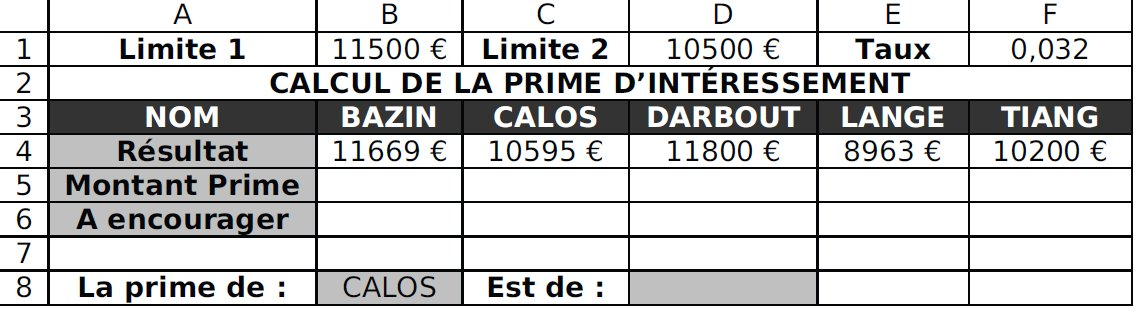
\includegraphics[width=0.7\textwidth]{exemple.jpg} 
\end{center}

\begin{enumerate}
 \item Proposez une formule (format Excel) permettant d'afficher dans la cellule B5 le montant de la prime \'egal au taux F1 appliqu\'e au r\'esultat B4 
 uniquement si celui-ci d\'epasse le montant ``Limite 1'' contenu dans la cellule B1.
 \item Proposez une formule permettant d'afficher dans la cellule D8 le montant de la prime du commercial dont le nom se trouve dans la cellule B8.
 \item Proposez une formule utilisant les fonctions INDEX() et EQUIV() permettant d'afficher automatiquement dans la cellule D8 le montant de la prime du commercial s\'electionn\'e en B8.
\end{enumerate}
% 
% \vspace{-0.3cm}
% \section{Utilisation de Wordpress}
% \vspace{-0.3cm}
% \exost (3 points) R\'epondez aux questions suivantes de mani\`ere concise.
% 
% \begin{enumerate}
%  \item Qu'est-ce qu'un syst\`eme de gestion de contenu (SGC) ou CMS?  % 1 point
%    \ifcorrection
%  \textcolor{red}{~\\Wordpress est un gestionnaire de contenu int\'egr\'e qui permet de d\'evelopper rapidement un site internet sans connaissance avanc\'ee en programmation.}
%  \fi 
%  %Quelles sont les principales diff\'erences entre un article et une page sous Wordpress?  %% 1pt
%  \item Expliquez quand il faut privil\'egier l'utilisation d'une \textbf{page} plut\^ot que d'un \textbf{article} sur Wordpress. Indiquez les principales diff\'erences entre un article et une page sous Wordpress? 
%  \ifcorrection
%  \textcolor{red}{~\\Un article est beaucoup plus complet qu'une page. Il permet de d\'evelopper un sujet en d\'etail, permettre aux lecteur de poster des commentaires. On choisira une page pour poster des informations statiques ou pour faciliter la navigation sur le site.}   % 3 point
%  \fi
%  \item Qu'est-ce qu'un \textit{shortcode} sous Wordpress? Expliquez leur utilit\'e et leur utilisation.  % 1 point
%    \ifcorrection
%  \textcolor{red}{~\\Un shortcode permet de placer des modules dans les pages sous wordpress.}
%  \fi 
% \end{enumerate}

\end{document}

% End Of File

